%%%%%%%%%%%%%%%%%%%%%%%%%%%%%%%%%%%%%%%%%%%%%%%%%%%%%%%%%%%%
%% introduction.tex
%%
%% Kapitel: Introduction
%% Autor: Axel Vierling (axel.vierling@cs.rptu.de)       
%% Autor: Jochen Hirth (j_hirth@informatik.uni-kl.de)       
%% Autor: Tobias Luksch (luksch@informatik.uni-kl.de)       
%% Datum: Juli 2003                                         
%%                                                          
%% Letzte Änderung Dezember 2023
%%%%%%%%%%%%%%%%%%%%%%%%%%%%%%%%%%%%%%%%%%%%%%%%%%%%%%%%%%%%
\chapter{Structure of the Document}
\label{chap:structure}
Here are some guidelines and recommendations to consider when creating the document. This section focuses more on the structural organization of the work rather than syntactical issues as addressed previously.

Foremost recommendation: It's crucial to consult with your supervisor early and frequently, especially regarding aspects like the structure and actual scientific content. This approach might save you some effort and time and provide assurance that you are on the right track, avoiding potential misdirection.

%%%%%%%%%%%%%%%%%%%%%%%%%%%%%%%%%%%%%%%%%%%%%%%%%%%%%%%%%%%%
\section{Thesis}
\label{sec:structure:thesis}
The most common structure of a thesis, valid for both master or bachelor theses usually looks like this
\begin{itemize}
    \item Introduction --- Here the topic should be introduced, and the structure, goal and scope of the thesis should be defined. One should focus on answering the following question: Why is the topic of the Thesis interesting for the (scientific) community?
    \item Background --- The main focus of this chapter should be to introduce everything that is needed to understand the further concepts of the thesis. This should entail everything you had to learn to understand and implement the task, and shortly cover the courses in your specialization you needed to understand the topic. The goal is to enable a reader from the same study program potentially from another specialization to understand the thesis.
    \item Related Work --- This question should answer the question: How did others try to solve the problem, and what did they miss? So, why is the problem not yet solved? In short, this should define the research gap of your work. For this, state-of-the-Art approaches should be described.
    \item Concept \& Implementation --- This is the first main part of the thesis. Here the approach you and your supervisor decided on should be explained. Usually, first on a higher level and then in detail including implementation details. So the question that is answered is: How do you try to solve the problem at hand?
    \item Experiments --- This is the second main part of the thesis. The experiments should be suitable to validate your approach. Define the experimental setting, e.g. the robot or the dataset, the metrics as well as the results. The visualization of the results should be in a way such that it is easily understandable. Usually, first, the results are reported and then the effects of the results on the defined problem are discussed. Answer the question, what parts of the problem did you solve?
    \item Conclusion \& Future Work --- Here the approach should be discussed related to the initial scope and goal. Answer the questions: What did you solve and especially what did you \textbf{not} solve? Give hints for potential extensions as future work.
\end{itemize}

%%%%%%%%%%%%%%%%%%%%%%%%%%%%%%%%%%%%%%%%%%%%%%%%%%%%%%%%%%%%
\section{Project}
\label{sec:structure:project}
The structure of a project is usually quite similar to the thesis, see Section~\ref{sec:structure:thesis}. As the scope is smaller, the Background and Related Work chapters are combined into one. But the exact structure depends more strongly on the task of the project.

%%%%%%%%%%%%%%%%%%%%%%%%%%%%%%%%%%%%%%%%%%%%%%%%%%%%%%%%%%%%
\section{Seminar}
\label{sec:structure:seminar}
The structure of the seminar again depends greatly on the topic -- and the supervisor. Here is however a general concept. Again, it is somewhat similar to Section~\ref{sec:structure:thesis}
\begin{itemize}
    \item Introduction --- Here the topic should be introduced, and the structure, goal and scope of the thesis should be defined. One should focus on answering the following question: Why is the topic of the Thesis interesting for the (scientific) community?
    \item Background --- The main focus of this chapter should be to introduce everything that is needed to understand the further concepts of the thesis. This should entail everything you had to learn to understand and implement the task, and shortly cover the courses in your specialization you needed to understand the topic. The goal is to enable a reader from the same study program potentially from another specialization to understand the thesis.
    \item State-of-the-Art Overview --- Answer the following questions: What different approaches exist to solve the problem? What do they do similar? What are the differences? What is the remaining research gap? All of this should be answered concisely, often best in a table. This should give a broad overview of the papers you read in your initial phase and summarize the overall topic. 
    \item Detailed-Concepts --- Here usually one or two approaches should be discussed in detail. Describe the key elements and how they solve the problem. More then 2 approaches can not be discussed in enough detail.
    \item Conclusion --- Here the results of the seminar should be summarized.
\end{itemize}

Instead of the here presented Top-Down approach also a Bottom-Up seminar report can be done, where chapters 3 and 4 are swapped.

\section{Dissertation}
\label{sec:structure:dissertation}
See Figure~\ref{fig:diss_structure}

\begin{figure}
    \begin{center}
      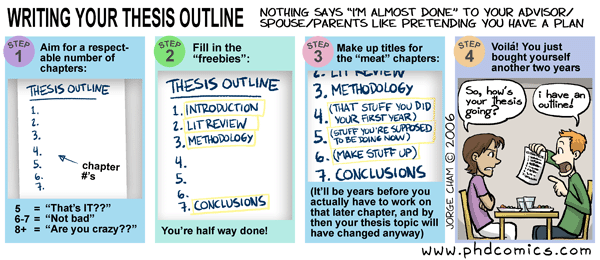
\includegraphics[width=15cm]{Diss_Structure}
      \caption{Common disserstation structure, see \url{https://phdcomics.com/comics/archive.php?comicid=715}}
      \label{fig:diss_structure}
    \end{center}
  \end{figure}


%%% Local Variables: 
%%% mode: latex
%%% TeX-master: "howto"
%%% End: 
